\chapter{Les états variables}
\section{Les champs en régime sinusoïdal permanent}
	\subsection{Les équations de Maxwell}	
	Si le milieu est linéaire et que la fréquence est fixée il  n'y aura pas de modification 
	de la fréquence et tous les champs oscilleront à celle-ci. En un point $\vec{r}$, le champ 
	électrique polarisé en $x$ varie selon
	\begin{equation}
	\vec{E}(\vec{r},t) = E_x(\vec{r},\omega)\cos(\omega t + \phi_x(\vec{r},\omega))\vec{1_x}
	\end{equation}
	On peut écrire ça sous forme de phaseur. Seule différence: le phaseur est un \textbf{vecteur 
	complexe} : $\underline{\vec{E}}(\vec{r},\omega) = \underline{E}_x(\vec{r},\omega)\vec{1_x}$.
	Bien sûr, il faudrait normalement considérer les trois composantes :
	\begin{equation}
	\underline{\vec{E}} = \underline{E}_x(\vec{r},\omega)\vec{1_x}+\underline{E}_y(\vec{r}
	,\omega)\vec{1_y}+\underline{E}_z(\vec{r},\omega)\vec{1_z}
	\end{equation}
	On peut également définir les phaseurs suivant :$\underline{\vec{B}}(\vec{r},\omega), 
	\underline{\vec{J}}(\vec{r},\omega)$ et $\underline{\vec{\rho}}(\vec{r},\omega)$. L'avantage 
	est que les équations de Maxwell deviennent algébriques
	\begin{equation}
	\begin{split}
	\rot \underline{\vec{E}}(\vec{r},\omega) &= -j\omega\underline{\vec{B}}(\vec{r},\omega)\\
	\rot \underline{\vec{B}}	(\vec{r},\omega) &= \mu\underline{\vec{J}}(\vec{r},\omega) +
	j\omega\epsilon\mu\underline{\vec{E}}(\vec{r},\omega)\\
	\div \underline{\vec{B}}(\vec{r},\omega) &= 0\\
	\div \underline{\vec{E}}(\vec{r},\omega) &= \dfrac{\underline{\rho}(\vec{r},\omega)}{\epsilon}
	\end{split}
	\end{equation}
	Ce système couple le champ électrique et magnétique. Exprimons sous forme intégrale la 
	première équation (intégration sur la surface)
	\begin{equation}
	\int_S \rot \underline{\vec{E}}(\vec{r},\omega)\ .\ \vec{dS} = -j\omega\int_S\underline{
	\vec{B}}(\vec{r},\omega)\ .\ \vec{dS}
	\end{equation}
	Par le théorème de Stokes :\\
	\retenir{\textbf{\ Loi de Faraday en phaseur}
	\begin{equation}
	\oint_C \underline{\vec{E}}(\vec{r},\omega)\ .\ \vec{dl} = -j\omega\int_S\underline{
	\vec{B}}(\vec{r},\omega)\ .\ \vec{dS}	
	\end{equation}
	À toute variation temporelle du champ magnétique est associé un champ électrique.}\ \\
	
	De même, pour la seconde équation
	\begin{equation}
	\int_S \rot\underline{\vec{B}}	(\vec{r},\omega)\ .\ \vec{dS} = \mu\underbrace{\int_S \underline{
	\vec{J}}(\vec{r},\omega)\ .\ \vec{dS}}_{=\underline{I}} + 	j\omega\epsilon\mu\int_S\underline{
	\vec{E}}(\vec{r},\omega)\ .\ \vec{dS}
	\end{equation}
	Par le théorème de Stokes\\
	\retenir{\textbf{\ Loi d'Ampère en phaseur}
	\begin{equation}
	\oint_C \underline{\vec{B}}	(\vec{r},\omega)\ .\ \vec{dl} = \mu\underline{I} + 
	j\omega\epsilon\mu\int_S\underline{\vec{E}}(\vec{r},\omega)\ .\ \vec{dS}
	\end{equation}
	À tout courant ou à toute variation temporelle du champ électrique, est associé un champ 
	magnétique.}
	
	\subsection{Résolution des équations de Maxwell}
	A part si la géométrie le permet, il est plus simple de passer par la méthode des potentiels 
	retardés. Montrons que si $\underline{\vec{J}}(\vec{r},\omega)$ est le phaseur associé à la 
	densité de courant, alors
	\begin{equation}
	\underline{\vec{J}}(\vec r,\omega)e^{-j\beta|\vec{r}-\vec{r'}|}
	\end{equation}
	où $\beta = \omega/c$ est le nombre d'onde, est le phaseur associé à la densité de courant 
	\textbf{retardée}. En effet
	\begin{equation}
	\begin{split}
	\Re\left(\underline{\vec{J}}(\vec{r},\omega)e^{-j\beta|\vec{r}-\vec{r'}|}e^{j\omega t}\right) &=
	\Re\left(\underline{\vec{J}}(\vec{r},\omega)e^{j\omega t - j\frac{\omega}{c} |\vec{r}-\vec{r'}|}
	\right)	 \\
	&=\Re \left(\underline{\vec{J}}(\vec{r},\omega)e^{j\omega\left(t-\frac{|\vec{r}-\vec{r'}|}{c}\right)}
	\right)\\
	&= \vec{J}\left(\vec{r},t-\dfrac{|\vec{r}-\vec{r'}|}{c}\right)
	\end{split}
	\end{equation}
	Ceci montre que l'exponentielle implique bien ce retard : chaque $e^{j\beta\clubsuit}$ modélise 
	le délai de propagation jusqu'à ce $\clubsuit$. En suivant un même raisonnement pour $\underline{
	\rho}$,  on peut écrire l'expression phaseurs des potentiels retardés\\
	
	\retenir{\begin{equation}
\underline{V}(\vec{r}) = \frac{1}{4\pi\epsilon_0}\int_\mathcal{D}\underline{\rho}(\vec{r'})\frac{e^{-j\beta|\vec{r}-
\vec{r'}|}}{|\vec{r}-\vec{r'}|}dV',\qquad
\underline{\vec{A}}(\vec{r}) = \frac{\mu_0}{4\pi}\int_\mathcal{D}\underline{\vec{J}}(\vec{r'})\frac{e^{-j\beta|\vec{r}-\vec{r'}|}}{|\vec{r}-\vec{r'}|}dV'
\end{equation}}

	En phaseurs, on obtient (à une constante près) les potentiels en intégrant les sources 
	multipliées par le \textbf{propagateur} (ou \textit{fonction de Green})
	\begin{equation}
	G(\vec{r},\vec{r'}) = \dfrac{e^{-j\beta|\vec{r}-\vec{r'}|}}{|\vec{r}-\vec{r'}|}
	\end{equation}
	Si l'on connaît la densité en $\vec{r'}$ et qu'on la désire en $\vec{r}$, il suffira juste 
	de la multiplier par le propagateur qui va décrire comment l'effet se manifestera jusque là 
	(ce n'est pas instantané. Remarquons qu'en statique ceci vaudrait 1 et on retrouverait la 
	fonction de Green de l'électrostatique). Le dénominateur sera justifié plus loin. En bref
	\begin{equation}
	e^{-j\beta|\vec{r}-\vec{r'}|}
	\end{equation}
	modélise le délai de propagation entre $\vec{r'}$ et $\vec{r}$.\\
		\exemple{Considérons une ligne de courant. Avec le précédent chapitre, on peut calculer le 
	courant en tout point et en déduire $\underline{J}$. On peut faire de même pour $\underline{
	\rho}$. Par intégration avec le propagateur, on peut calculer $\underline{V}$ et $\underline{
	A}$ en tout point et donc $\underline{E}$ et $\underline{B}$.}
	
	
	\subsection{La jauge de Lorentz}
	Si l'on effectue une étude des dimensions de notre problème, nous pouvons nous rendre compte 
	que nous avons un degré de liberté de moins que ce nous pouvions penser : c'est là qu'intervient 
	la théorie des jauges, où le cas de l'électromagnétisme est le prototype le plus simple de 
	cette théorie\footnote{Merci à Philippe Grégoire pour l'explication complémentaire.}.\\
	\retenir{\ \textbf{Jauge de Lorentz}
	\begin{equation}
	\vec{\nabla}\ .\ \underline{\vec{A}}(\vec{r},\omega) = -j\omega\mu_0\epsilon_0\underline{V}(\vec{r},
	\omega)
	\end{equation}}\ \\
	
	En calculant cette jauge, on peut tout déduire : elle permet de se passer de l'équation du 
	potentiel scalaire (on peut obtenir $\underline{V}$ à partir de $\underline{\vec{A}}$ et 
	qui plus est de façon plus simple). La démonstration n'est pas à connaître.
	
\section{Application : l'effet pelliculaire}
À haute fréquence $\vec{J}$ n'est plus constante au sein d'une section de fil. Comme nous 
sommes ici dans un cas \textit{très académique}, le plus simple est de passer par les équations 
de Maxwell et d'appliquer $\vec{J} =\sigma\vec{E}$ :
\begin{equation}
\rot\vec{\underline{B}}(\vec{r},\omega) = \mu\sigma\vec{\underline{E}}(\vec{r},\omega) + j\omega
\mu\epsilon \vec{\underline{E}}(\vec{r},\omega)
\end{equation}
Or $\epsilon \ll \sigma$ $\left(\text{En effet : }\ \frac{\sigma}{\omega\epsilon}\approx\frac{10^{1
8}}{f}\right)$ : le terme de conduction est bien supérieur au terme de courant de déplacement 
que l'on négligera ici. Il faut alors résoudre
\begin{equation}
\begin{split}
\oint_C \vec{\underline{E}}(\vec{r},\omega)\ .\ \vec{dl} &= -j\omega\int_S \vec{\underline{B}}
(\vec{r},\omega)\ .\ \vec{dS}\\
\oint_C \vec{\underline{B}}(\vec{r},\omega)\ .\ \vec{dl} &= \mu\sigma\int_S \vec{\underline{E}}
(\vec{r},\omega)\ .\ \vec{dS}
\end{split}
\end{equation}
Pour montrer que les deux champs sont liés, nous allons ici faire un raisonnement itératif. 
Soit un courant selon $z$ et $E_0$ la valeur du champ électrique au centre de la section. À 
très basse fréquences
\begin{equation}
\vec{\underline{E}} = E_0\vec{1_z}
\end{equation}

	\begin{wrapfigure}[7]{l}{5.15cm}
	\vspace{-5mm}
	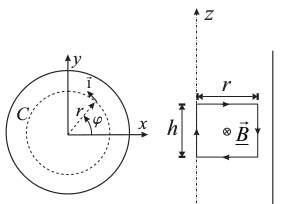
\includegraphics[scale=0.45]{ch3/image1.png}
	\captionof{figure}{ }
	\end{wrapfigure}
Ce champ est forcément associé à un champ d'induction, disons $\vec{\underline{B}}=\vec{B_0}$. 
En considérant un contour ampérien circulaire
\begin{equation}
\begin{array}{lll}
\DS \oint_C \vec{B_0}\ .\ \vec{dl} &=\DS \oint_C B_0\vec{1_\varphi}\ . \vec{1_\varphi}\ dl &= 2\pi 
r\ B_0\\
\DS\mu\sigma\int_S = E_0\vec{1_z}\ .\ \vec{dS} &=\DS \mu\sigma\int_S E_0\vec{1_z}\ .\ \vec{1_z}\ dS 
&= \mu\sigma \pi r^2 E_0
\end{array}
\end{equation}
Dès lors $\vec{\underline{B}} = B_0\vec{1_\varphi} = \frac{\mu\sigma}{2}rE_0\vec{1_\varphi}$. Or 
le champ d'induction magnétique varie, Faraday doit être vérifiée. Or, en remplaçant cette 
expression dans celle de la loi de Faraday cela ne fonctionne pas. Le champ électrique postulé 
n'est pas correct, il faut lui apporter un terme correcteur lorsqu'on s'éloigne du centre (et 
donc nul en $r=0$):
\begin{equation}
\vec{\underline{E}} = (E_0+E_1(r))\ \vec{1_z}
\end{equation}
Appliquons la loi de Faraday en choisissant un contour rectangulaire :
\begin{equation}
\oint_C (E_0+E_1(r))\ \vec{1_z}\ .\ \vec{dl} = -j\omega\int_S\underline{\vec{B}}(r)\ .\ \vec{dS}
\end{equation}
où la contribution du terme constant est nul $\oint_C E_0\vec{1_z} . \vec{dl}=0$. Il reste pour le membre de
gauche
\begin{equation}
\oint_C E_1(r)\vec{1_z}\ .\ \vec{dl} = \int_0^h \underbrace{E_1(0)}_{=0}\vec{1_z}.\vec{1_z}\ dz +
\int_0^h E_1(r)\vec{1_z}.(-\vec{1_z})\ dz = -hE_1(t)
\end{equation}
Pour le membre de droite, nous avons
\begin{equation}
-j\omega \int_S \vec{\underline{B}}(\vec{r},\omega)\ .\ \vec{dS} = -j\omega \int_0^h\int_0^r 
B_0(r)\vec{1_\varphi}.\vec{1_\varphi}\ dr\ dz = -j\omega h\dfrac{\mu\sigma}{2}E_0\dfrac{r^2}{2}
\end{equation}
On trouve un terme correctif dépendant de la fréquence
\begin{equation}
E_1 = j\omega\dfrac{\mu\sigma}{4}r^2E_0
\end{equation}
Rebelote, il faut recalculer $B$ comme $E=E_0$ a été modifié : $\vec{\underline{B}} = (B_0(r)+
B_1(r))\vec{1_\varphi}$. De façon similaire, on trouve
\begin{equation}
B_1=j\omega\dfrac{(\mu\sigma)^2}{16}r^3E_0
\end{equation}
Rerebelote, il faut calculer un terme $E_2(r)$ correctif dans l'expression de $\vec{\underline{E}}$, 
\dots Après un certains nombre d'itération, on trouve
\begin{equation}
\begin{split}
\vec{\underline{E}} &= \DS E_0\left(1+j\dfrac{\omega\mu\sigma}{4}r^2-\dfrac{(\omega\mu\sigma)^2}{64}r^4
+\dots\right)\vec{1_z}\\
&= \DS E_0\left(1-\dfrac{\gamma^2r^2}{4}+\dfrac{\gamma^4r^4}{64}+\dots\right)\vec{1_z}
\end{split}
\end{equation}
où $\gamma^2=-j\omega\mu\sigma$. Cette série tend vers la fonction de Bessel d'ordre 0, $J_0$ :
\begin{equation}
\vec{\underline{E}} = E_0J_0(\gamma r)\vec{1_z}
\end{equation}
En remarquant, $a$ étant distance entre le centre et la surface du fil, $\vec{\underline{E}}(a) = E_0J_0(\gamma a)\vec{1_z}$, on écrit\\

\retenir{\begin{equation}
\vec{\underline{E}}(r) = \dfrac{J_0(\gamma r)}{J_0(\gamma a)}\underline{\vec{E}}(a)
\end{equation}}\ \\

Le comportement asymptotique à haute fréquence ($\gamma r \rightarrow\infty$) de la fonction de 
Bessel est disponible dans les tables. On peut, en développant $\gamma$, trouver:\\
\retenir{\textbf{\ Profondeur de peau}\begin{equation}
\delta = \sqrt{\dfrac{2}{\omega\mu\sigma}}
\end{equation}}\ \\

À  haute fréquence, on obtient finalement\footnote{Les détails sont donné page 53, mais ils 
ne sont pas physiquement intéressants.} 
\begin{equation}
J_0(\gamma r) \approx \sqrt{\dfrac{1}{2\pi\gamma r}}e^{jr/\delta}e^{r/\delta}e^{-j\pi/4}
\end{equation}
Ceci montre que proche de la surface du fil, le courant évolue exponentiellement.

\newpage
	\begin{wrapfigure}[10]{r}{5.5cm}
%	\vspace{-5mm}
	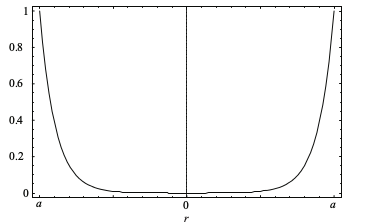
\includegraphics[scale=0.45]{ch3/image2.png}
	\captionof{figure}{ }
	\end{wrapfigure}
Nous remarquons sur le schéma ci-contre que proche du centre, il n'y a pas de courant. Pour une 
certaine valeur, en s'approchant de la périphérie, le courant "explose". On peut considérer 
que le courant n'existe que dans une pellicule d'épaisseur $\delta$. Cet effet n'est pas 
négligeable (\SI{50}{\hertz} :$\delta = \SI{9}{\milli\meter}$. \SI{100}{\mega\hertz} : $\delta = \SI{6}{\micro\meter}$). Cet effet est d'autant plus 
important car la résistance apparente n'est pas celle à considérer. Par exemple, dans les 
câbles coaxiaux, les courants "seulement superficiels" voient leur résistance augmentée avec le 
carré de la fréquence
\begin{equation}
R_1 = \dfrac{1}{\sigma\delta}\left(\dfrac{1}{2\pi a}+\dfrac{1}{2\pi b}\right)=
\sqrt{\dfrac{\omega\mu}{2\sigma}}\left(\dfrac{1}{2\pi a}+\dfrac{1}{2\pi b}\right)
\end{equation}
Pour le fun, l'expression du champ électrique à haute fréquence, non valable au centre (
$\gamma r \rightarrow \infty)$ vaut 
\begin{equation}
\underline{\vec{E}}(r) \approx \vec{\underline{E}}(a)\sqrt{\dfrac{a}{r}}e^{-j\frac{a-r}{\delta}}
e^{-\frac{a-r}{\delta}}
\end{equation}
	
	
	
	
	
	
	
	
	
	
	
	
	
	
	
	
	